\section{Data}
\label{sec:data}

Between January 1st 2018 and January 1st 2019 samples of daily tweets were searched using the Observatory on Social Media (OSoMe; 48). OSoMe of the Indiana University Network Science Institute (IUNI) provides access to 10\% of tweets each day. To construct the cohorts OSoMe was searched using the query „diagnos*” as well as different specific internalizing disorder queries (e.g., „anxiety”, „OCD”, „depression”).  Based on the previously described inclusion approach (44, 49), social media users were gathered who have stated to have an actual clinical diagnosis of either anxiety or depression. An example statement would be „my doctor diagnosed me with depression”. Self diagnoses, such as „I must be depressed”, were excluded. Afterwards the gathered tweets were searched for the words „i”, „diagnos*”, „depres*/ anx*” in that order in a case-insensitive manner. to match the greatest variety of diagnosis statements. The queries were then combined to obtain the greatest variety of self-referential diagnosis statements within the tweets. 

The subjects were then grouped into an anxiety (A) cohort and a depression (D) cohort based on these statements about clinical diagnoses. All people who exhibited diagnoses for both anxiety and depression were excluded from the analyses.

Based on the results of a comparative analysis of social media sampling methods by Ernala et al (2019; „Methodological Gaps in Predicting Mental Health States from Social Media: Triangulating Diagnostic Signals.”) it was ensured that only self-referential tweets of a clinical diagnosis of either depression or anxiety were included. Thus, the remaining statements were assessed using three judges. They decided whether a tweet was self-referential and excluded perceived jokes, quotes or external references. Only statements that were unanimously rated as self-referential of a clinical diagnosis were kept in the dataset. As Chancellor and Choudhury (2019; „Methods in predictive techniques for mental health status on social media”) propose, conclusions in regards to depression’s population morbidity and its language features based on the use of data-driven supervised machine learning approaches were avoided. 

Using the Twitter „user\_timeline” API endpoint (https://developer.twitter.com/en/docs/tweets/timelines/api-reference/get-statuses-user\_timeline) the timeline for each Twitter user who has made a qualifying statement was gathered. All retweets and all tweets in a different language (i.e. non-English) were removed. Further, tweets posted before January 1st 2018 were excluded as they predate the diagnosis reference that was referred to. 

Lastly, to ensure that only accounts belonging to individuals were included, M3 and Botometer were used. M3 is a demographic classification algorithm assessing accounts to be an organization or institution. Similarly Botometer is a software identifying automated accounts (bots).

Some demographic information, while not usually publicly available for social media profiles, was estimated. Machine learning methods exist for estimating demographics from profiles online. For example, for this article, \textit{M3} \citep{m3} was used to predict a user's age and gender. It predicts a gender propensity for each user. If the probability of gender classification is greater than $80\%$, an individual is labeled as either male or female (Macro-F1: $0.915$). Age was classified into the cateogories “18 and below”, “19–29”, “30–39”, and “40 and up”. The model achieves a Macro-F1 of $0.425$ for age categorization.

\subsection{Inferring time zone information}

User activity on social media platforms such as Twitter is strongly influenced by the time of day. For instance, individuals tend to be significantly less active during nighttime hours when they are likely to be asleep, and more active during waking hours, typically corresponding to their local daytime. In datasets comprising globally distributed users, this diurnal variation necessitates accounting for users' time zones when analyzing temporal patterns of activity or sentiment. Failing to do so can obscure meaningful trends or introduce systematic biases into the analysis.

However, explicit time zone information is available for only a small fraction of users—specifically, 419 users in this dataset who have provided self-reported location data that could be reliably mapped to a time zone. To enable time-of-day-based analyses at scale, it becomes essential to infer the time zones of the remaining users. To address this, an inference algorithm was developed that leverages the temporal distribution of each user’s tweeting activity. By analyzing frequency distributions across UTC-based timestamps, the algorithm aims to estimate the most probable time zone for each user.

First, the 419 users with known time zones were used to construct a reference distribution of tweet activity. This distribution represents the proportion of tweets posted at each hour of the day, rounded to the nearest full hour. It served as a baseline pattern for identifying the most likely local time of activity.

For users without known time zones, their timestamps were systematically adjusted across all possible UTC offsets from -12 to +15 hours. For each possible offset, a new hourly distribution of tweet activity was computed. We selected the best offset by minimizing the mean absolute error (MAE) between the shifted distribution and the reference distribution.

To evaluate the effectiveness of this approach, the 419 users with known time zones were used as a test set, meaning their actual time zones were compared with the inferred ones. However, this introduced a degree of bias, as the reference distribution was derived from the same users being evaluated.

The results indicated that the algorithm exactly matched the correct time zone in only 19.33\% (0.1933) of cases. However, the accuracy improved when considering slight deviations: in 57.76\% (0.5776) of cases, the predicted time zone was within one hour of the correct value. The accuracy depending on tolerance level is visualized in Figure \ref{fig:time-zones}.

\begin{figure}
    \centering
    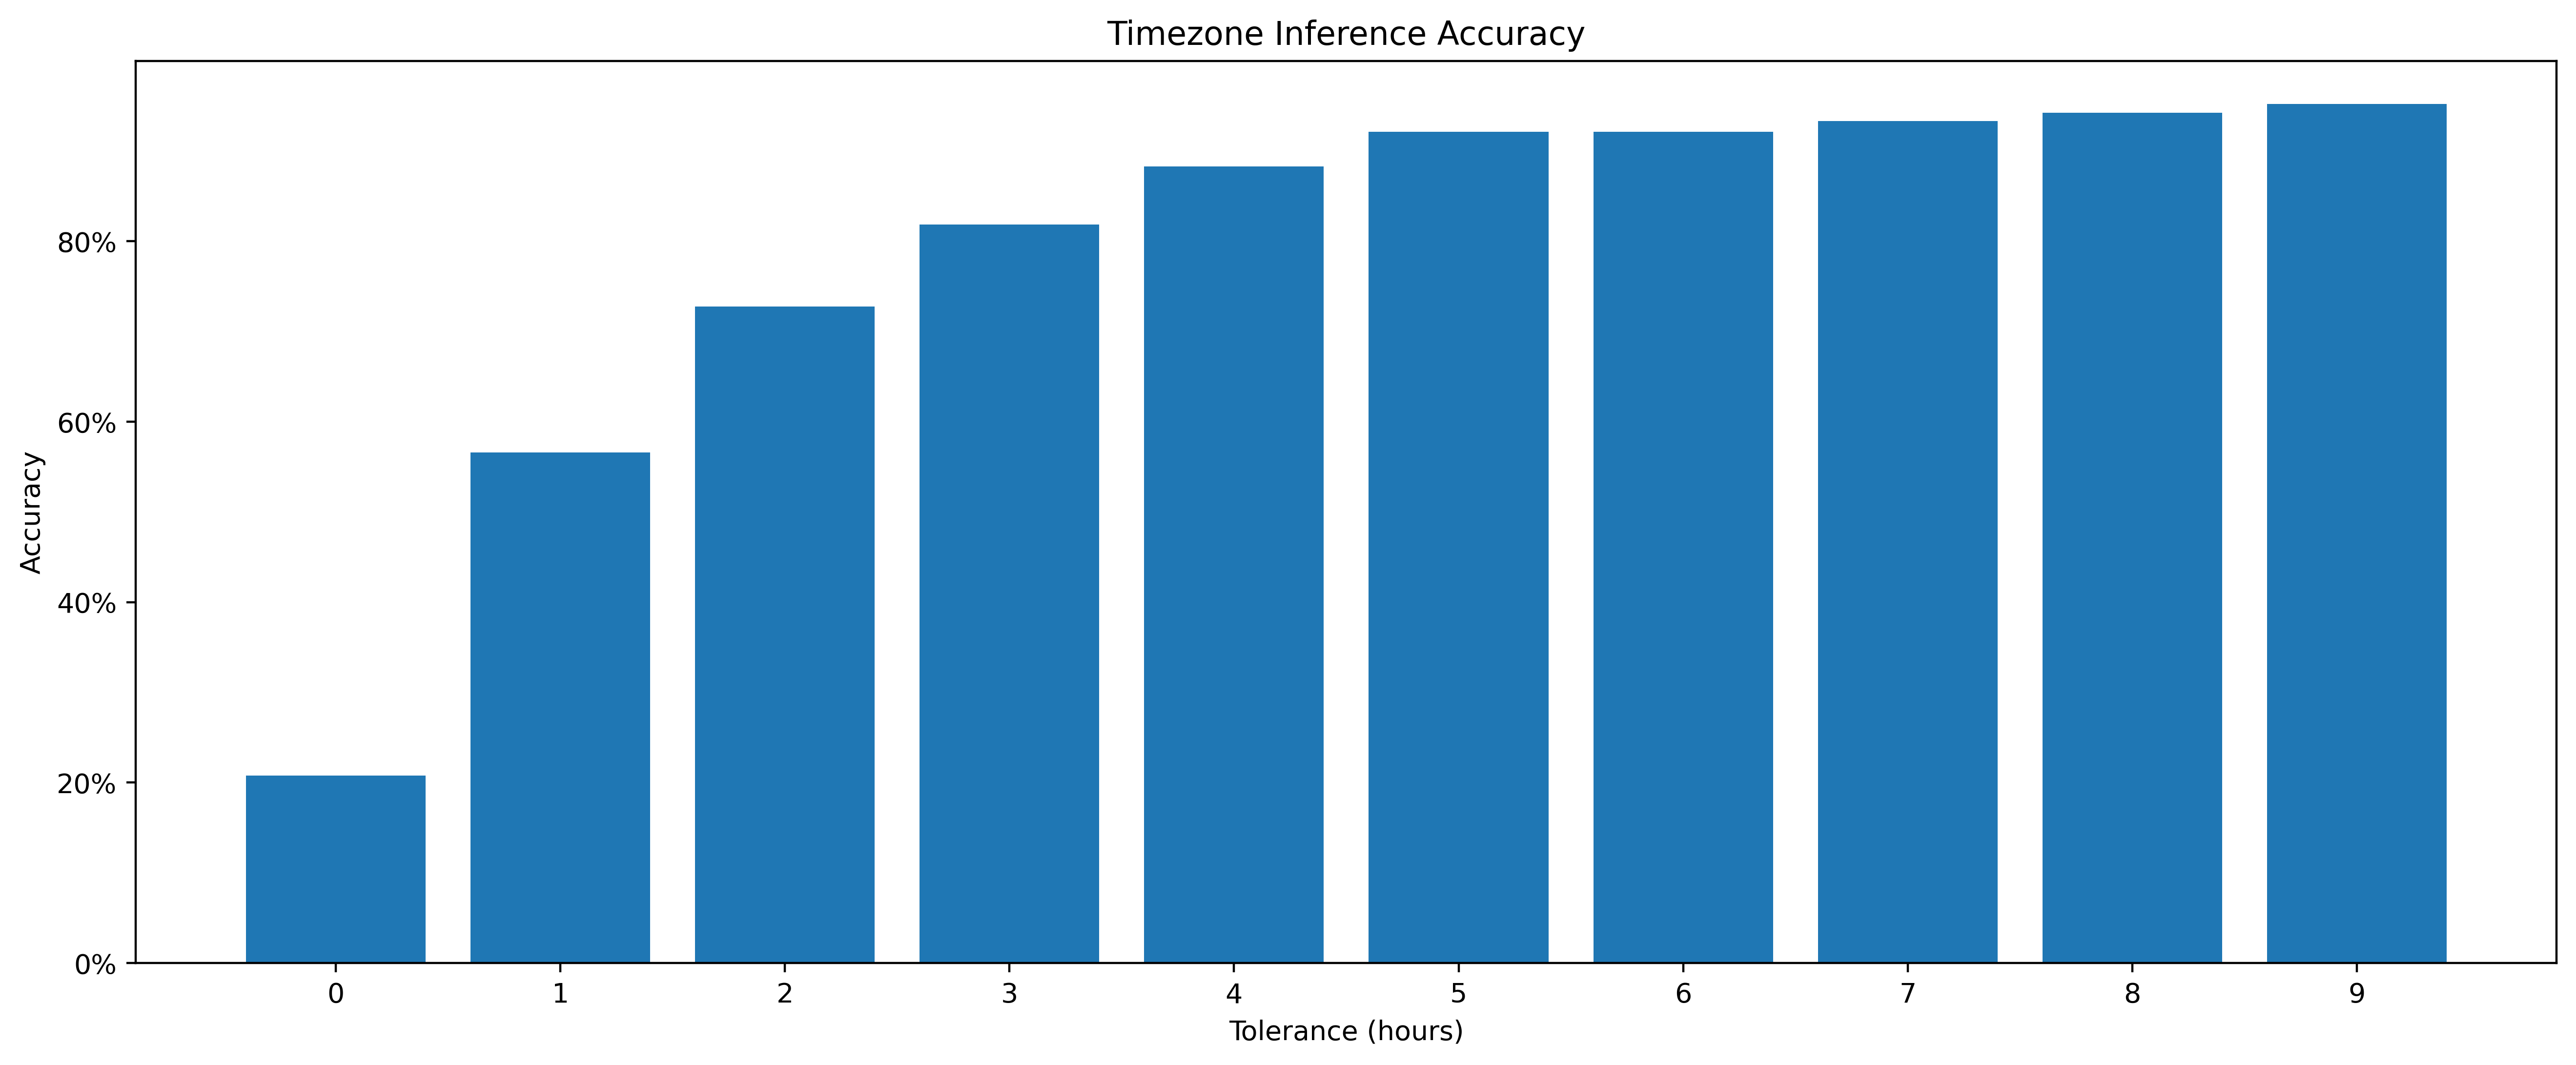
\includegraphics[width=\linewidth]{Images/timezone_inference_accuracy.png}
    \caption{Time zone inference accuracy by tolerance level in hours.}
    \label{fig:time-zones}
\end{figure}

While this method captures general tweeting patterns, it has notable limitations. User behavior varies significantly, and external factors such as work schedules, night shifts, or irregular online habits can distort the assumed daily tweeting rhythm. Additionally, the reliance on mean absolute error assumes that errors in hour misalignment are linearly penalized, which may not always reflect real-world consequences of incorrect time zone estimation.

This approach provides a reasonable approximation of users' time zones when explicit information is unavailable, leveraging behavioral patterns in tweet timing. However, the relatively low exact match rate suggests that further refinement is needed, potentially incorporating additional behavioral signals or machine learning techniques to improve predictive accuracy. These limitations ought to be taken into account when assessing the time of day based results.

For all users without explicit time zone information, the predicted time zone was used for all further analyses.


\subsection{Descriptives}

In total, the sample was made up of 1795 individuals who published 1172 tweets on average (IQR: $422 - 1684$) across the entire time span. Of the individuals for which the gender could be determined, 1218 were female, while only 560 were male. Thus, the dataset was heavily skewed towards women. Approximately 73.61 \% of users in the dataset were younger than 30 years old, with only 10.18 \% being older than 40. 

Demographic information for the users is reported in Table~\ref{tab:descriptives_subset_total}. 

\begin{table}[h]
    \caption{Descriptive statistics for all users included in the analyses.}
    \centering
    
    \begin{tabular}{ccccccccc}
        \hline
        Cohort & n & n female & avg. tweets (sd) & age $\leq 18$ & age $19-29$ & age $30-39$ & age $\geq 40$  \\
        \hline
        Depression & 1270 & 717 & 1182.74 (991.61) & 33.35\% & 40.62 \% & 15.38 \% & 10.53 \% \\
        Anxiety & 492 & 293 & 1169-93 (888.67) & 30.67\% & 41.81 \% & 18.87 \% & 8.65 \% \\
        \hline
    \end{tabular}
    
    \label{tab:descriptives_subset_total}
\end{table}


Most tweets were published during the week days, with Wednesday being the day with the most traffic. Saturday is the day on which the fewest tweets were set off (see Figure \ref{fig:tweets_by_dow}). 

\begin{figure}[h]    
    \centering
    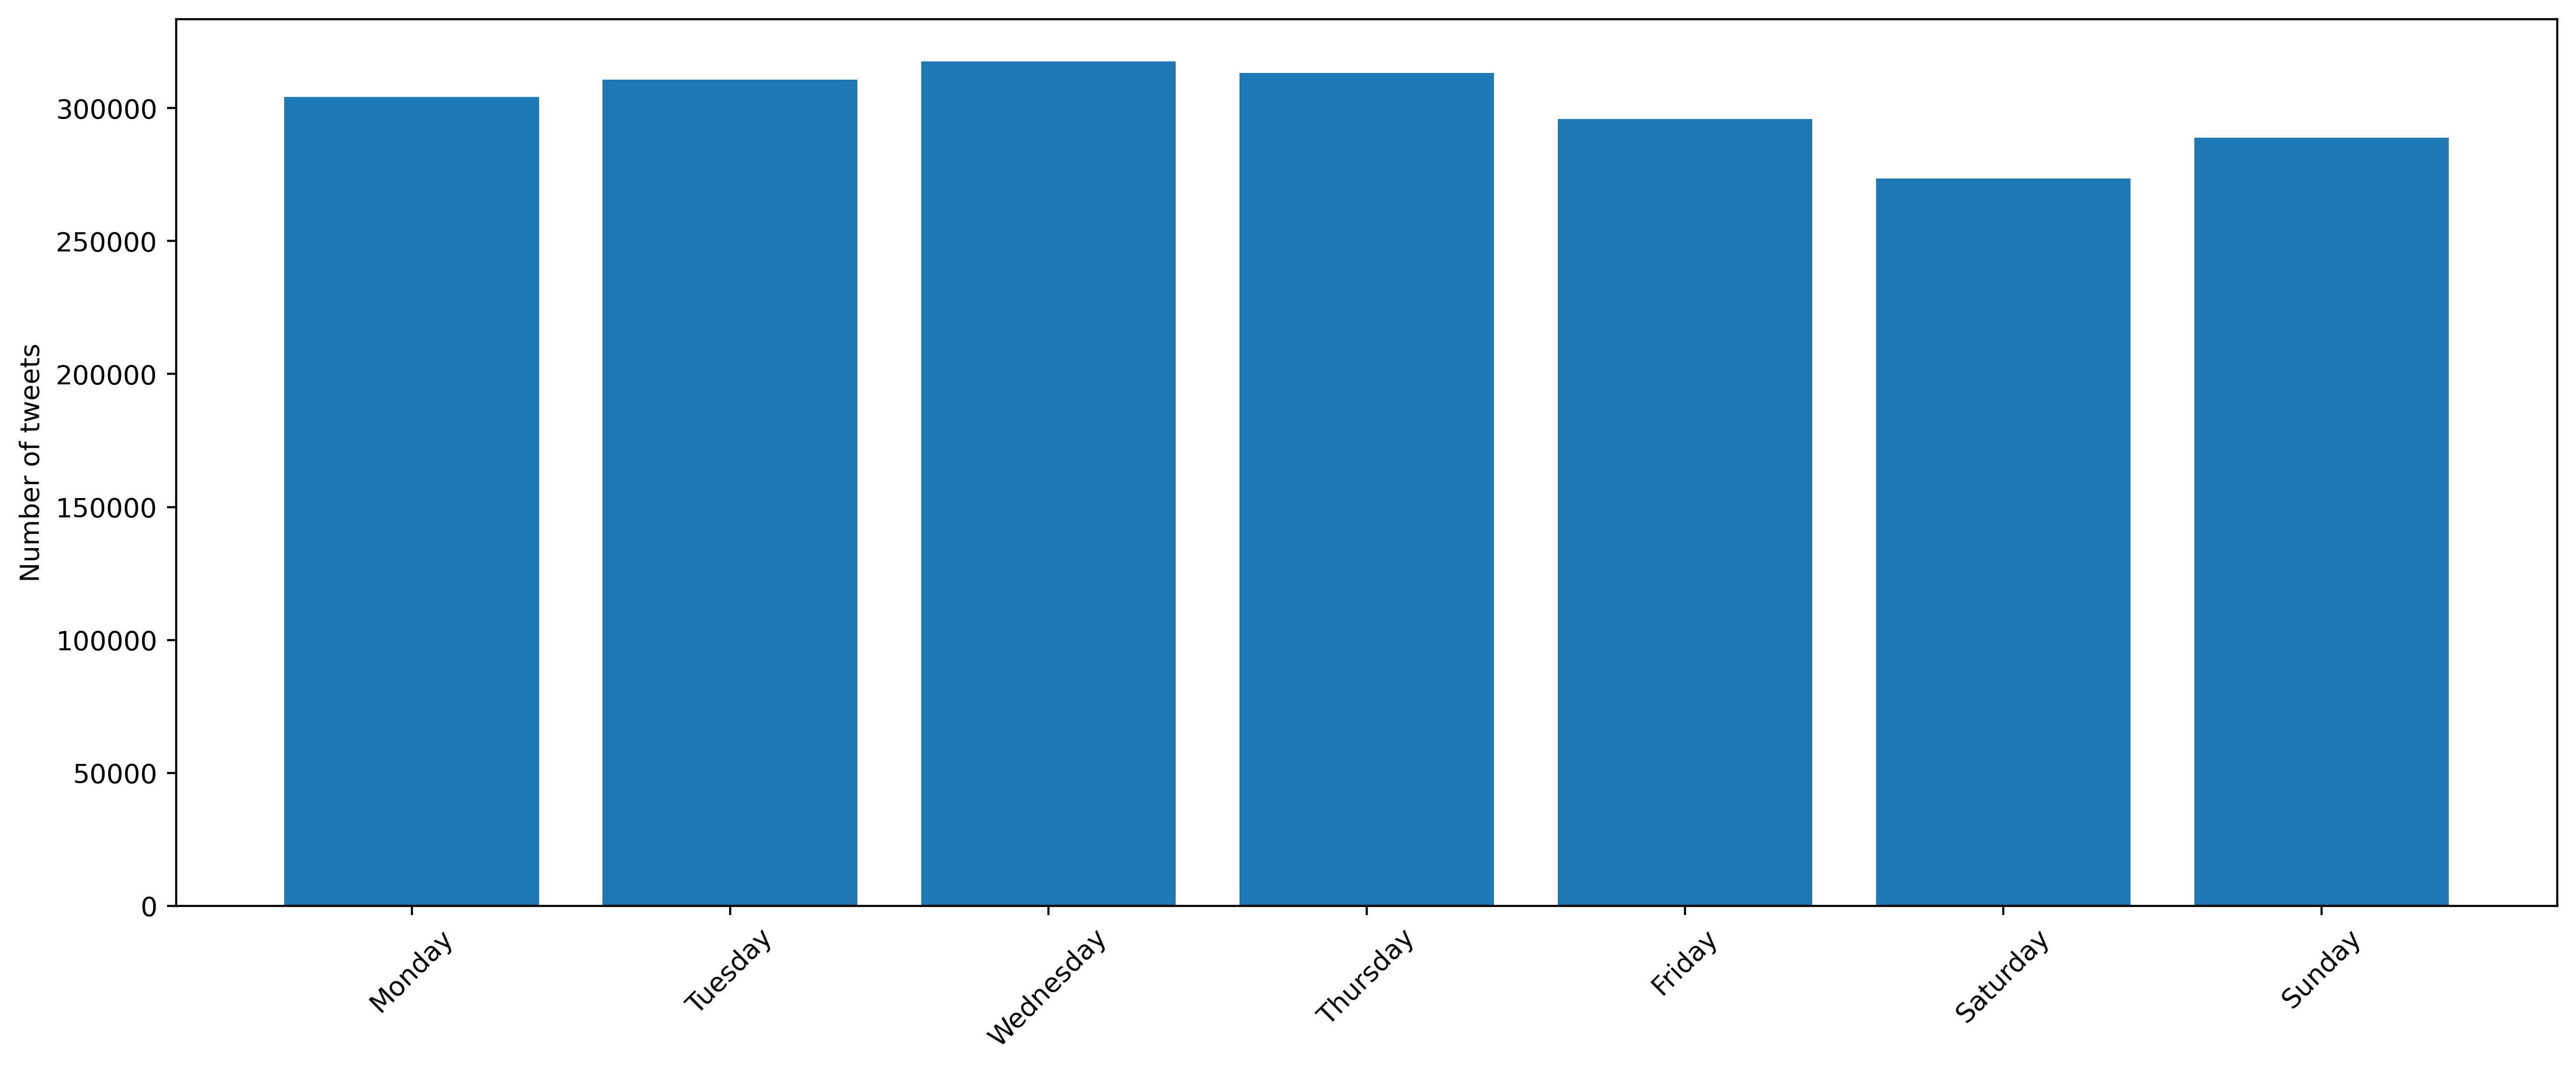
\includegraphics[width=\linewidth]{Images/tweets_by_dow.png}
    \caption{Number of published tweets by day of week}
    \label{fig:tweets_by_dow}
\end{figure}

\begin{figure}[h]
    \centering
    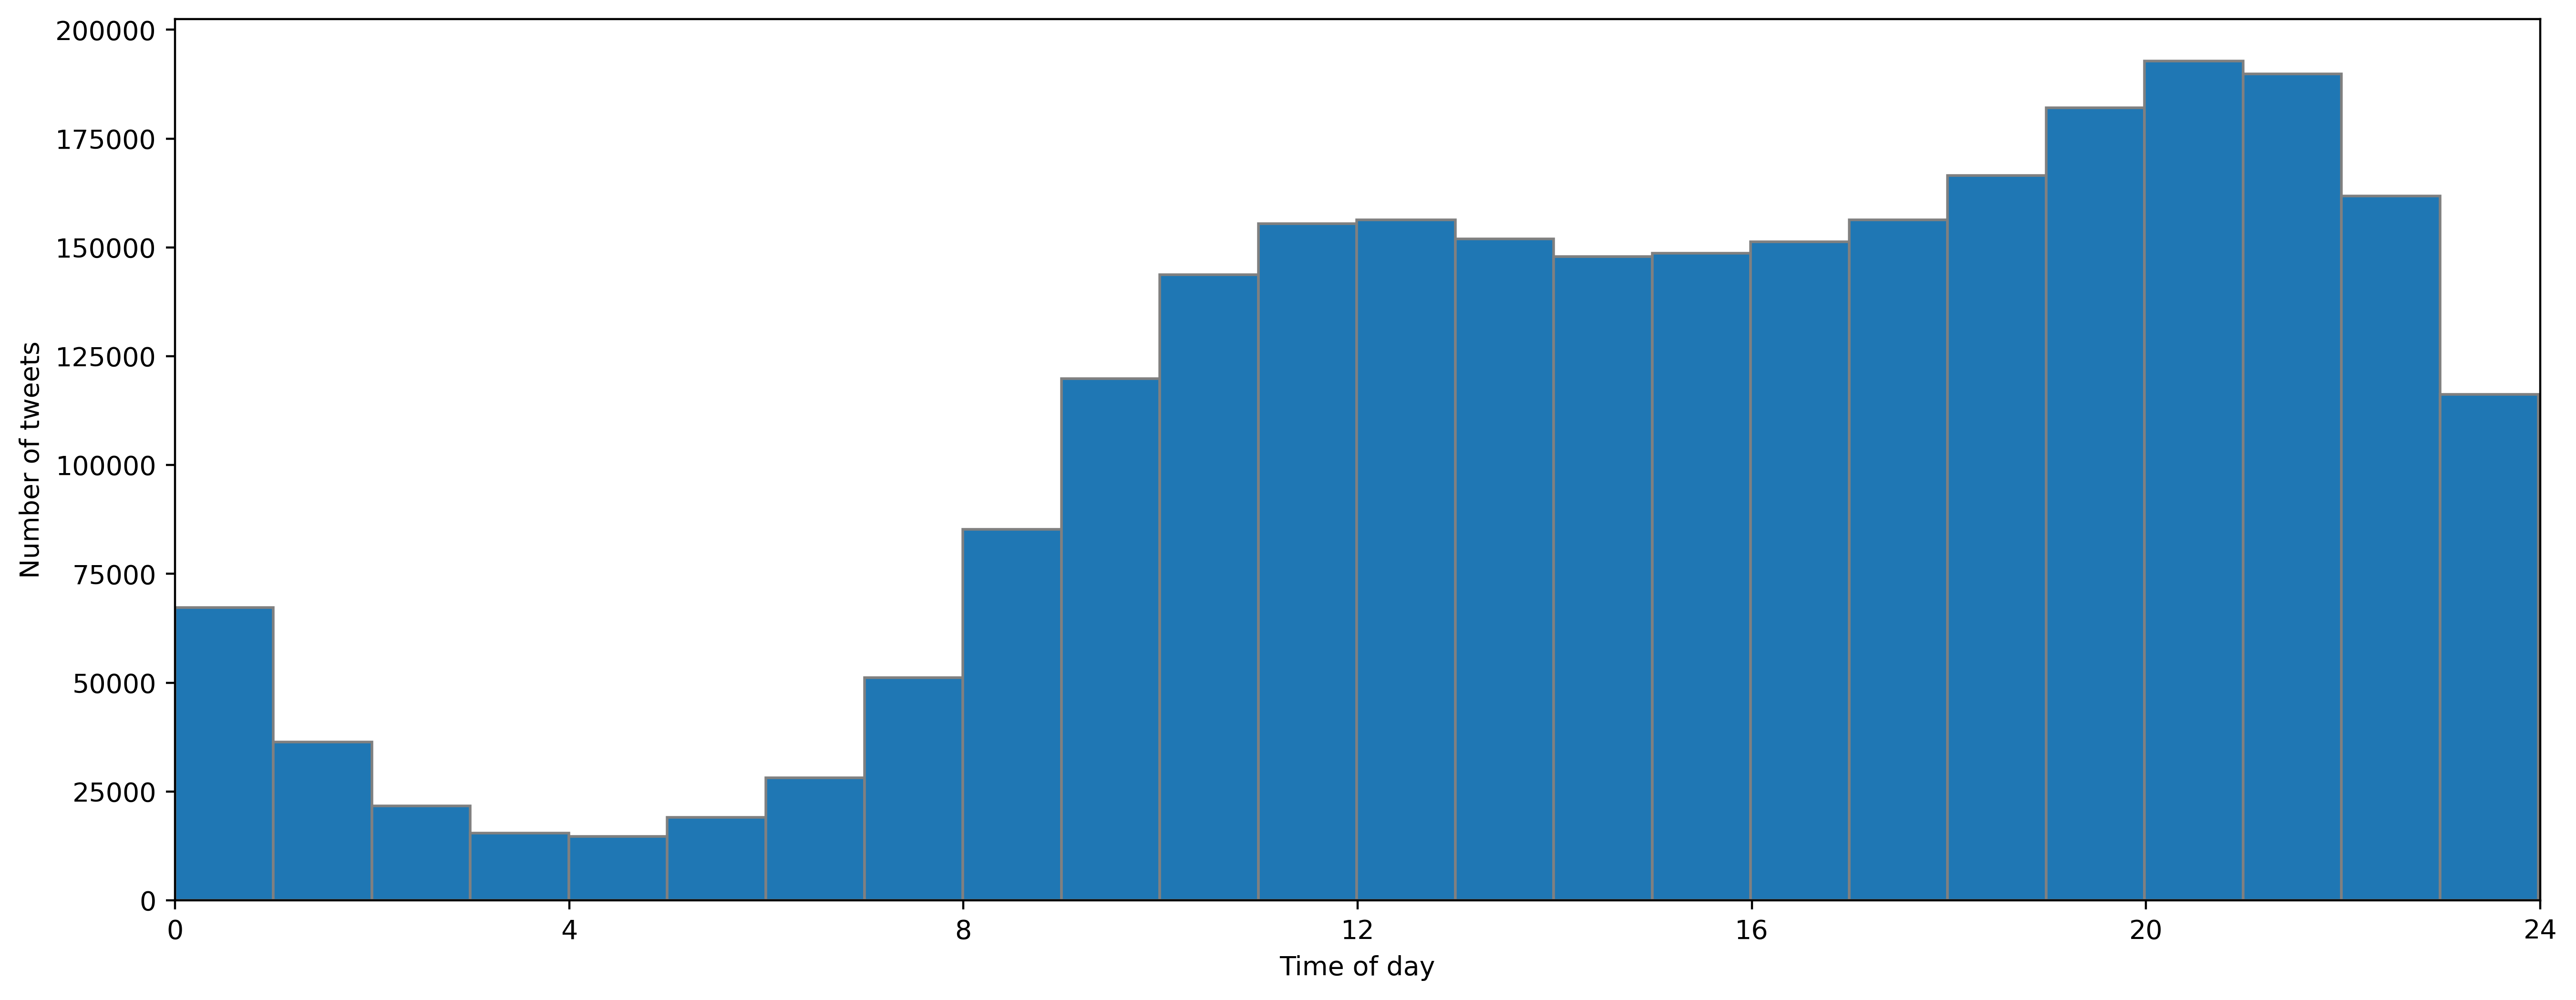
\includegraphics[width=\linewidth]{Images/tweets_per_hour.png}
    \caption{Number of published tweets by time of day}
    \label{fig:tweets_by_tod}
\end{figure}

\begin{figure}[h]
    \centering
    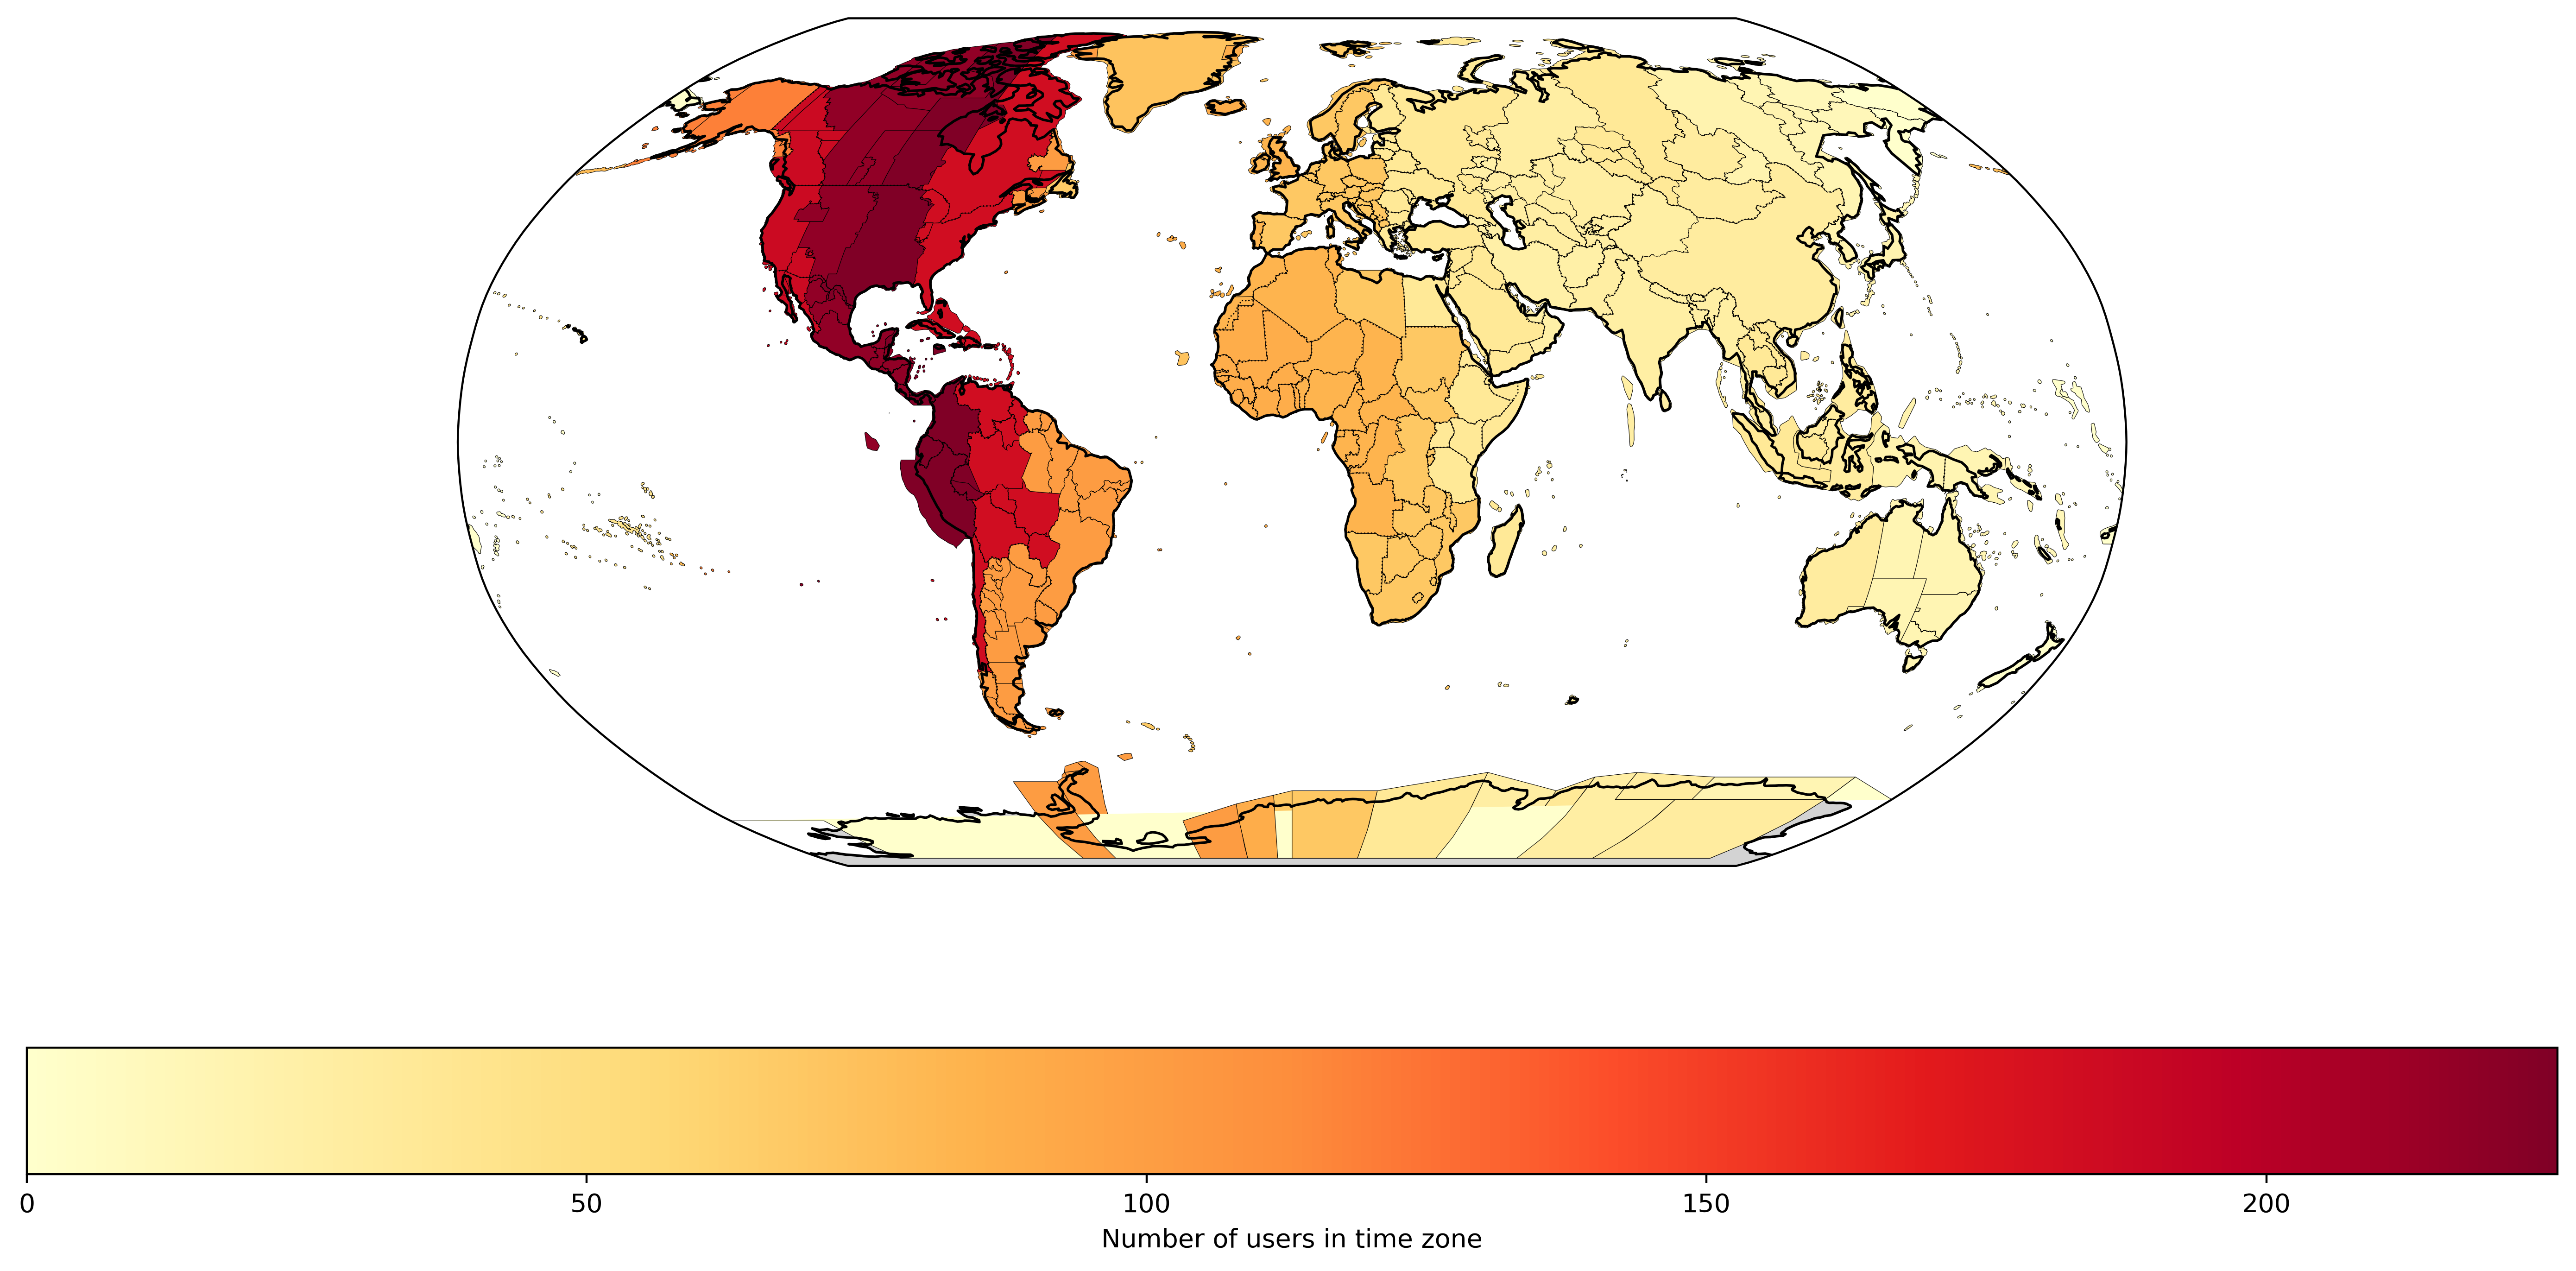
\includegraphics[width=\linewidth]{Images/timezone_frequencies.png}
    \caption{Number of users by time zone}
    \label{fig:timezone_distribution}
\end{figure}

The distribution of Twitter users across time zones, as depicted in Figure~\ref{fig:timezone_distribution}, revealed a clear concentration of users in specific UTC offsets. The map demonstrates a peak in user frequency around UTC \textit{-7} to UTC \textit{-4}, which corresponds to regions such as North America, particularly the Central Time Zones of the United States. A secondary concentration is observed around UTC \textit{0}, likely reflecting users from Western Europe. There appears to be little activity in Asia, indicating that most activity originated in the western hemisphere. This uneven distribution highlights the geographical bias in Twitter activity, which should be considered when analyzing temporal trends in sentiment or online behavior. This was likely influenced or even caused by filtering for English-only tweets.